\chapter{istar: Software as a Service}

Having released and advertised idock, we kept receiving constant docking requirements from our colleagues and collaborators. They are mostly biochemists and pharmacists, outsourcing the docking research to us after discovering potential biological targets for certain diseases of therapeutic interest. All of a sudden, we had to grab the protein structure, do format conversion, define search space, set up docking parameters, and keep running idock in batch for months. Tedious enough, all the above work was done manually, resulting in very low research productivity. Even worse, our idock process got killed by other users or by exceptions occasionally.

Originally motivated by the desire to automate the docking process, we then developed istar, a SaaS (Software as a Service) platform. Later on we realized that istar could be a general SaaS platform for any program, therefore in addition to idock \citep{1153}, we also managed to host our tool igrep \citep{1138}. Without tedious software installation, users, especially computational chemists, can submit jobs on the fly either by browsing our web site or by programming against our RESTful API. Figure \ref{istar:istar} shows the web site and the architecture of istar. Under typical circumstance, a user opens a browser and submits a job. The web server validates user input and saves it into database. Several workstations fetch jobs from the database and actually carry out the massive experiments. Upon completion, they send the user a completion notification email and write the result to a network file system, which is served as static content by the web server. The user again browses our web site to track progress and retrieve result.

\begin{figure}
\centering
\includegraphics[width=\linewidth]{istar/istar.png}
\caption{http://istar.cse.cuhk.edu.hk}
\label{istar:istar}
\end{figure}

On the client side, we seamlessly combined both the Twitter Bootstrap and the HTML5 Boilerplate into a HTML5- and CSS3-powered web site, which was successfully checked as HTML5 by the W3C Markup Validator v1.3. We adopted the \textit{de facto} jQuery library to simplify HTML document traversing, event handling, animating, and Ajax interactions, and the jQuery UI library to provide themeable widgets. We tested the web site with Chrome 19+, Firefox 12+, Internet Explorer 9+, Safari 5+ and Opera 12+, and utilized the Modernizr library to detect HTML5 and CSS3 features in order to maintain backward compatibility in older browsers.

On the server side, we built the web server in the same JavaScript language using the well-known asynchronous event-driven node.js on top of the express server, forking multiple worker processes to accept simultaneous HTTP/SPDY connections. We utilized the spdy node module to support SPDY protocol v3, the prototype of next generation HTTP 2.0. We employed the forever node module to restart worker processes automatically in case of unhandled exceptions, ensuring failover and high availability. We made use of regular expressions and developed a customized version of the validator node module to validate and sanitize user input upon job receival, ensuring data validity. We are considering prepending the scalable asynchronous event-driven nginx as a front-end HTTP server for a rich set of features, like bandwidth throttling, static file serving, reverse proxy for caching, load balancing, URL rewriting, gzip compression, TLS/SSL support, IP-based geolocation, etc.

On the database side, we chose MongoDB, a scalable, high-performance, open source NoSQL database. MongoDB features document store in JSON style, making it particularly suitable for applications requiring flexible document attributes like our istar. MongoDB is written in C++, making it easy to manipulate the database from idock and igrep, which are also written in C++. By using a 10gen-supported native MongoDB driver for node.js, the web server is able to save user input as jobs into MongoDB.

On the workstation side, we are maintaining a Linux workstation, equipped with Intel Xeon W3520 @ 2.66 GHz, 8GB DDR3 SDRAM and NVIDIA GeForce GTX 285 (1024 MB), and running a minimal version of Fedora 17 x64. Meanwhile, from our department we have exclusively reserved 4 Mac workstations, equipped with Intel Core i5 2400 @ 3.10GHz and 4GB DDR3 SDRAM, and running Mac OS X Lion 10.7.4 Build 11E53. We are collaborating with Mr. Frank Ng at ITSC on purchasing a HP s6500 4U Chassis server with 8 NVIDIA Tesla M2090 6GB.

On the network file system side, we mounted a 2TB hard disk for shared use. All the 5 workstations can simultaneously access to the hard disk and perform file reading and writing. In principle, we will persist existing jobs and results until storage shortage.

As for software availability, similar to idock, istar is also hosted at GitHub for version control and freely available at https://github.com/HongjianLi/istar. Its source code is licensed under the Apache License 2.0 while its documentation is licensed under CC BY 3.0.

\section{idock on istar}

Eventually we managed to interconnect every component and host idock \citep{1153} on istar. The was exactly our first and foremost motivation of constructing istar.

On the client side, figure \ref{istar:idock} shows the web site of idock. The upper section displays information about existing jobs, including the number of ligands to dock, submission date, current status and progress, and result for download. Client-side paging is supported, and an Ajax timer is started to automatically refresh the status and progress in real time by quering against the web server every second. The lower section allows new job submission. A new job typically consists of several compulsory fields as well as several optional fields. Compulsory fields include a receptor in PDBQT format, a search space defined by a cubic box, a short job description, and an email to receive completion notification. Optional fields include 9 ligand filtering conditions, like molecular weight, partition coefficient xlogP, apolar desolvation, polar desolvation, number of hydrogen bond donors, number of hydrogen bond acceptors, topological polar surface area tPSA, net charge, and number of rotatable bonds. We set up default values for optional fields, and only the ligands satisfying all the 9 filtering conditions will be docked. Figure \ref{istar:idock-rest} shows the RESTful API of idock. We expose the functionalities of job submission, job query, and ligand counting as RESTful API for others to program against.

\begin{figure}
\centering
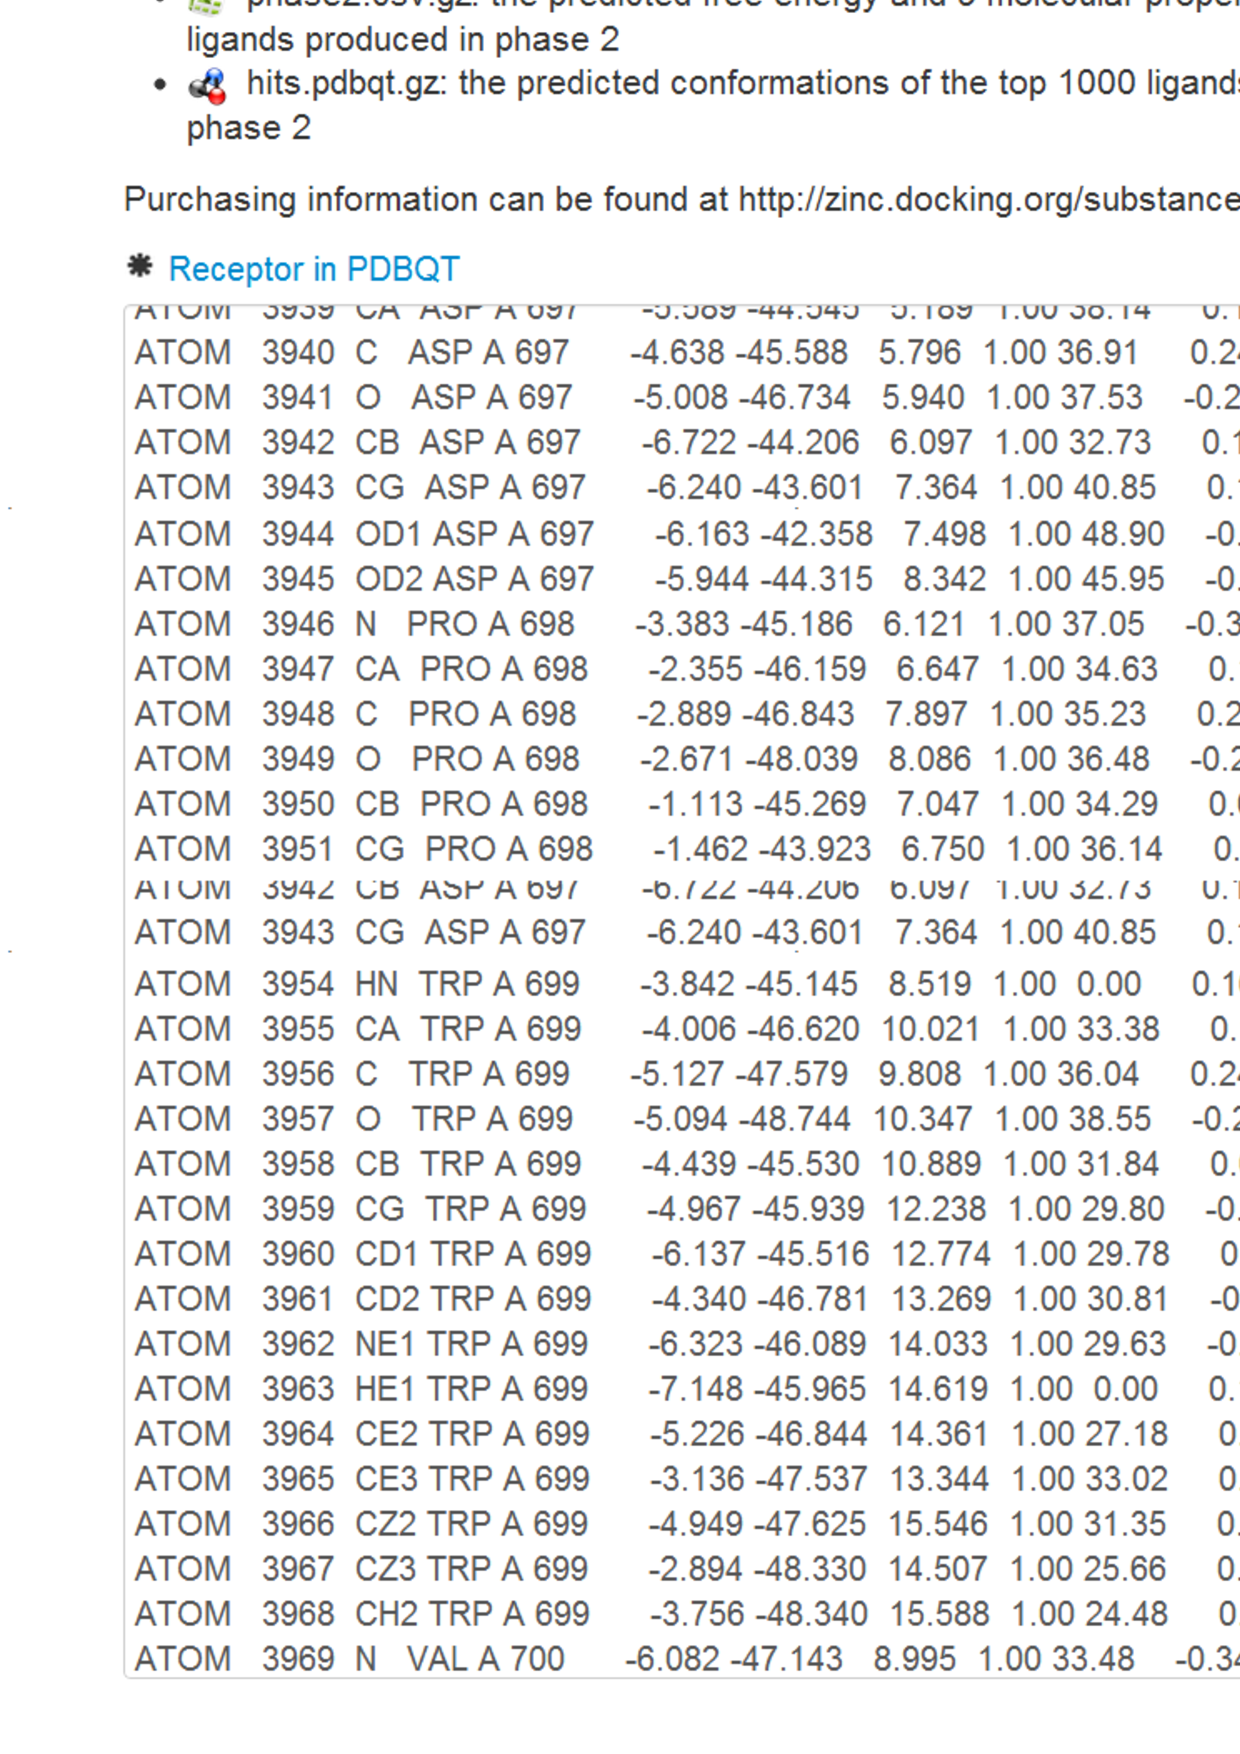
\includegraphics[width=\linewidth]{istar/idock.png}
\caption{http://idock.cse.cuhk.edu.hk}
\label{istar:idock}
\end{figure}

\begin{figure}
\centering
\includegraphics[width=\linewidth]{istar/RESTfulAPI.png}
\caption{RESTful API of idock.}
\label{istar:idock-rest}
\end{figure}

On the server side, during startup, the master process loads and parses 9 molecular properties of 12 million ligands (Figure \ref{istar:LigandProperties}), and awaits queries from worker processes through inter-process message passing. Upon receival of a query from a worker process, the master process performs an in-memory table scan and calculates the number of ligands satisfying a given combination of filtering conditions on those 9 molecular properties. The ligand count is signaled to the query-invoking worker process and then forwarded to the client side. The entire round trip costs approximately one second, rendering the feasibility of real-time ligand counting queries for users to estimate in advance how many ligands will be docked. Originally we stored the 9 molecular properties in MongoDB, but our in-house trial showed that it took about 9 seconds to complete a ligand counting query even in the presence of index and even having the data stored in a RAM disk. Disappointed by the poor performance of MongoDB given 12 million documents, we decided to abandon this design and let the master process hold the data in memory throughout its lifecycle.

\begin{figure}
\centering
\subfloat
{
  \includegraphics[width=0.315\linewidth]{istar/MWT.pdf}
}
\subfloat
{
  \includegraphics[width=0.315\linewidth]{istar/LogP.pdf}
}
\subfloat
{
  \includegraphics[width=0.315\linewidth]{istar/Desolv_apolar.pdf}
}
\\
\subfloat
{
  \includegraphics[width=0.315\linewidth]{istar/Desolv_polar.pdf}
}
\subfloat
{
  \includegraphics[width=0.315\linewidth]{istar/HBD.pdf}
}
\subfloat
{
  \includegraphics[width=0.315\linewidth]{istar/HBA.pdf}
}
\\
\subfloat
{
  \includegraphics[width=0.315\linewidth]{istar/tPSA.pdf}
}
\subfloat
{
  \includegraphics[width=0.315\linewidth]{istar/Charge.pdf}
}
\subfloat
{
  \includegraphics[width=0.315\linewidth]{istar/NRB.pdf}
}
\caption{Distributions of 9 molecular properties of the 12,171,187 clean ligands.}
\label{istar:LigandProperties}
\end{figure}

On the network file system side, we collected 12,171,187 clean ligands at pH 7 in mol2 format from the fruitful ZINC database \citep{532,1178} with explicit permission of its major developer and maintainer, Prof. John J. Irwin at University of California, San Francisco. Originally the yuck-compound-free ligands are organized into 98 slices, with each slice containing approximately 125,000 clean ligands, among which about 75,000 (60\%) have a molecular weight of at least 350g/mol (Figure \ref{istar:gt350}), the minimum weight requirement that a modern drug should bear. We converted all the 12 million ligands into PDBQT format in batch, and combined the 12 million individual files and integrated their 9 molecular properties into one single file as huge as 50GB for subsequent parallel docking. The format conversion alone required 2 months. We also recorded and encoded the offset of each ligand within that big file for fast random seeking.

\begin{figure}
\centering
\includegraphics[width=\linewidth]{istar/gt350.pdf}
\caption{Distributions of ligands whose molecular weight is above 350g/mol of the 98 slices.}
\label{istar:gt350}
\end{figure}

On the workstation side, we developed a customized version of idock as a daemon in modern C++11, adding necessary code to iteratively fetch a pending job slice from MongoDB, reuse receptor and grid maps whenever possible, perform 2-phase docking, report progress to MongoDB, and send email notification upon job completion.

On one hand, the idock on istar features 2-phase docking (Figure \ref{istar:2PhaseDocking}), due to as many as 12 million ligands to screen. In phase 1, idock performs coarse but fast virtual screening without writing any conformations to file, aiming to quickly shortlist a few thousand candidate compounds. In phase 2, idock performs fine but slow virtual screening with a significantly larger number of Monte Carlo tasks per ligand, writing as many conformations to file as possible and aiming to refine the predicted free energy as well as predicted conformation of candidate compounds. Such a 2-phase docking methodology can remarkably reduce job execution time while avoiding the risk of filtering out potentially promising compounds, controlling the false negative rate at an acceptable level.

\begin{figure}
\centering
\includegraphics[width=\linewidth]{istar/2PhaseDocking.png}
\caption{istar 2-phase docking.}
\label{istar:2PhaseDocking}
\end{figure}

On the other hand, the idock on istar features slice-level parallelism in phase 1. Generally speaking, multiple workstations can compete for either jobs or slices, with the former known as job-level parallelism and the latter as slice-level parallelism (Figure \ref{istar:2LevelParallelism}). Job-level parallelism is very straightforward to implement and can ensure high utilization of computational power when the number of jobs exceeds the number of workstations. Nevertheless, when the number of workstations exceeds the number of jobs, which is usually the case in practice during the initial stage of istar, slice-level parallelism can better utilize computational power by subdividing a job into slices which are then distributed to workstations. Slice-level parallelism is, in contrast, difficult to implement on both the database side and the workstation side. The technical hurdle becomes even more apparent when results from multiple workstations must be properly combined to produce a final result and progresses from multiple workstations must be properly combined too to compute an overall progress. Finally we succeeded in splitting a job into 100 slices and distributing them to idle workstations in phase 1 to achieve parallel docking.

\begin{figure}
\centering
\subfloat[Job-level parallelism.]
{
  \label{istar:JobLevelParallelism}
  \includegraphics[width=\linewidth]{istar/JobLevelParallelism.png}
}
\\
\subfloat[Slice-level parallelism.]
{
  \label{istar:SliceLevelParallelism}
  \includegraphics[width=\linewidth]{istar/SliceLevelParallelism.png}
}
\caption{istar 2-level parallelism.}
\label{istar:2LevelParallelism}
\end{figure}

Together with 2-phase docking as well as slice-level parallelism, using a Mac workstation alone, on average it takes a week to complete one single slice. Therefore, even though we thoroughly utilize all the 4 Mac workstations, it can take up to 5 months to complete one single job. Currently we have 3 jobs at hand, adding up to 15 months, and we believe more jobs are coming in the future. In order to boost job execution and expect a speed up of at least an order of magnitude, we plan to port idock to GPU using both CUDA and OpenCL/WebCL in both C++ and JavaScript and deploy new workstations equipped with high-end GPU chips.

\section{igrep on istar}

In the beginning, we constructed istar specifically as an online version of idock. We never realized it could become a general SaaS platform until the day we borrowed a GeForce GTX 680 from ITSC. With such a high-end graphics card at hand, we wanted to try something out. My own program igrep \citep{1138} escaped my mind. igrep was developed two years and is a fast CUDA implementation of agrep algorithm for approximate nucleotide sequence matching. Then I spent three weeks rewriting the entire code, porting igrep to istar, and upgrading 26 genomes for instant search.

Figure \ref{istar:igrep} shows the web site of igrep. The workflow is more or less identical to idock. New jobs are submitted via browsers and validated by our web server. They are stored into the database and subsequently distributed to the sole Linux workstation for execution. Figure \ref{istar:igrep-rest} the RESTful API, allowing job query and submission.

\begin{figure}
\centering
\includegraphics[width=\linewidth]{istar/igrep.png}
\caption{http://igrep.cse.cuhk.edu.hk}
\label{istar:igrep}
\end{figure}

\begin{figure}
\centering
\includegraphics[width=\linewidth]{istar/RESTfulAPI.png}
\caption{RESTful API of igrep.}
\label{istar:igrep-rest}
\end{figure}

igrep is not our focus, but the success of hosting it on istar tells us two things: istar can host any program, and can utilize GPU acceleration.

\chapterend
